%===========================================================
%                              Choix de thématique
%===========================================================
% Une des quatre options 'parallelisme', 'architecture', 'systeme' 
% 'tempsreel' doit être utilisée avec le style compas2021
\documentclass[systeme,french,english]{compas2022}
\usepackage[utf8]{inputenc}

\usepackage{algorithm2e}
\usepackage[T1]{fontenc} %% Vector fonts
\usepackage[numbers,square,sort&compress]{natbib} %% Better bibliography
\usepackage{parskip} \parskip=1ex plus 5pt minus 1pt \parindent=4ex %% indent paragraphs
\usepackage{xspace}  %% Macros with automatic spacing
\usepackage[defblank]{paralist}  %% inline lists
%===========================================================
%                               Title
%===========================================================

\toappear{1} % Conserver cette ligne pour la version finale

\begin{document}
\selectlanguage{english}

\title{Towards correct high-performance database systems}
\shorttitle{Correct High-Performance DBMSs}

\author{Saalik Hatia(1), Annette Bieniusa(2), Carla Ferreira(3), Gustavo Petri(4), Marc Shapiro(1)}


\address{
  (1)~LIP6--Sorbonne-Université, Paris, France  \\
  (2)~TU Kaiserslautern, Germany \\
  (3)~Universidade NOVA de Lisboa, Portugal \\
  (4)~ARM, Cambridge, United Kingdom\\
  }

\date{\today}

\maketitle

%===========================================================         %
%R\'esum\'e
%===========================================================  
\begin{abstract}
  Our goal is to design and implement a full-featured, high-performance
  geo-distributed database that is correct by construction.
  We adopt a stepwise approach.
  We start from a simplistic concurrent database system; we formalise an
  operational semantics and its key invariants; we also provide a
  reference implementation and test cases exercising the invariants.
  From there, we plan to prove that the semantic model satisfies the
  invariants (proof in Coq), and to check that the implementation respects
  the model thanks to litmus-test cases.
  Each following step adds a single feature.
  We formalise the feature, and expect to show formally and experimentally
  that the improved system simulates the simpler one.
  We expect that the features compose, so that the correctness of the full
  system with all the features follows from the individual proofs.
  At the time of writing, the operational semantics for several steps is
  complete; the translation to Coq and the reference implementation are
  ongoing.

  \MotsCles{
    système réparti,
    base de données géo-distribuée,
    vérification formelle,
    test
    }
\end{abstract}

\tableofcontents

%=========================================================
\section{Introduction}
%=========================================================

Modern online applications use a distributed database management
system (DDBMS), to provide users with available and consistent data.
The purpose of a DDBMS is conceptually simple: to store and retrieve
shared data.
However, for performance and fault-tolerance reasons, the internals of a
typical database are very complex, with many moving parts that interact
in hard-to-understand ways.
Existing databases are designed in a manual and ad-hoc manner;
inevitably, they have bugs that impact the consistency and integrity of
data.

The goal of this work is to build a database that is correct by design,
while including some important optimisations (e.g., caching)
and properties (e.g., fault tolerance).
Formalising a database that provide users with fast read and writes,
data safety and geo-replication is hard.
Any attempt to verify at once some monolithic specification, including
all the interesting properties, is probably doomed to failure.
Instead, we propose the following incremental approach,  decompose the
system into a set of small, orthogonal modules and features.

Our starting baseline is a bare-bones and ``obviously correct'' DDBMS,
restricted to its simplest function, i.e., transactions reading and
writing data.
We formalise its operational semantics and specify its invariants.
We prove (in Coq) that the semantics satisfies the invariants.
We also provide a (hand-written) reference implementation, and use test
cases derived from the formal model to check that it follows the
semantics and does not violate the invariants.

Each design step adds a single feature, e.g., a cache or logging,
with its associated operational semantics and invariants.
We use simulation (or bisimulation) to show that the formal model is
equivalent without and with the feature, modulo the added constraints.
We take a similar approach with the reference implementation.
Furthermore, we compare performance without and with the feature.

Our ultimate aim is to show that the final design, including all the
features, is both correct (by simulation of the baseline) and has
comparable performance to ad-hoc database systems with similar features.
We claim that providing developers with a clear model helps to implement
a correct, high performance and geo-distributed database.

\section{Transactions and timestamps}
\label{sec:transactions}

A client of the DDBMS executes transactions.
Classically, a transaction is a sequence of reads and updates, bounded by
a begin and an end.
The transaction either aborts with no effects; or it commits and all its
commits become visible atomically to later transactions.
Formally, the choice between abort and commit is non-deterministic (in
practice it depends on the application's invariants and on external
events, such as sufficient resources being available).

We formalise the mutual ordering of transactions with abstract
\emph{timestamps}.
Committing a transaction $i$ assigns it a commit timestamp
$\mathit{Ct}_{i}$; all its updates are labelled with this commit
timestamp.
Conversely, a transaction $j$  has a \emph{snapshot timestamp} (or dependency
timestamp) $\mathit{Dt}_{j}$.
Transaction $i$ precedes transaction $j$ if $\mathit{Ct}_{i} \le
\mathit{Dt}_{j}$.
Transaction $j$ \emph{depends on} all transactions $i$ such $i$ precedes
$j$; any read that $j$ performs includes all the updates with a label
less or equal to $\mathit{Dt}_{j}$.
The set of such preceding updates is called the \emph{snapshot} of
transaction $j$.
 
Our formalisation is agnostic to the transaction model (e.g.,
serialisable or snapshot-isolation).
For space reasons, this paper considers a single model, Transactional
Causal Plus Consistency (TCC+), i.e., causal consistency with
transactions and convergence \cite{rep:syn:sh228,rep:pro:sh182}.
Under TCC+, a snapshot must be a causally-consistent cut.
Other transaction models differ by timestamp ordering being partial or
total, and by constraints on beginning and committing a transaction.

The formal model represents a transaction with the following information:
\begin{compactitem}
\item $\tau$: unique transaction identifier.
\item $\mathit{Dt}$: dependency timestamp.
\item {$\varepsilon$}: effect map, records the updates made by the transaction.
\item ${R}$: read set, records the objects read by the transaction.
\item $\mathit{Ct}$: commit timestamp, assigned if and when the
  transaction commits.
\item $\mathit{State}$: status, either \emph{not\_started}, \emph{live} or \emph{terminated}.\\
\end{compactitem}

A Read updates the read set $R$; a write updates the effect map $\varepsilon$.


\subsection{Timestamps and snapshots}

We use timestamps as method of concurrency control.
Every transaction has a timestamp (Ct) that is assigned by the system when the transaction is committed.
It is used to perform arbitration on the order of the transactions.

Using these timestamps we define a snapshot as a collection of transaction that have a commit timestamp less than or equal to a timestamp.
The latter is called the Dependency Snapshot Timestamp.

Snapshots provide \emph{isolation} guarantees to the system, meaning a client only reads object versions that are part of the snapshot and are committed. 
In addition to isolation, snapshots also provide the client with \emph{atomicity} guarantees: $\varepsilon_i$ of a transaction $\tau_i$ are seen in an all-or-nothing manner.

\subsection{Object-version}

Having only one version of an object severly limits concurrency in a database.
Multi-Version Concurrency Control (MVCC) is a technique that allows a database to have multiple versions of an object (Object-Versions).
Every update to an object creates its own version and to ensure that all transactions read the correct version of an object the system maintains the following information: 
\begin{itemize}
  \item \emph{key} is the unique identifier of the object.
  \item \emph{$\tau_i$} identifier of the transaction that wrote this version.
  \item \emph{blob} is a pointer to the value of the materialized object.
\end{itemize}

In this paper we note object-version by $(key ,\tau_i)$.

% \section{Approach}

% Our ultimate goal is to arrive at a database that has a Journal for fast writes, a Checkpoint Store that enable truncation of the journal and speed up reads and recovery and is distributed for geo-replication.

% We have two choices to start from:
% \begin{itemize}
%   \item An in-memory key-value store that stores operations in a sequential Journal.
%   \item An in memory key-value store that create and store states.
% \end{itemize}

% To start we do not impose any constraints on the size of the memory footprint.
% This allow use to focus only on transaction handling and the invariants that are associated with them.
% From there we can add either fault tolerance by adding a persistency layer or restrict the amount of memory used by the database.
% The different transitions are represented in figure 1 \ref{fig:transitions}.

\section{System Model}

Starting from a simple in memory Key-Value store, we describe the model then progressively add features and compare every progression between them (\emph{figure \ref{fig:transitions}}).
We provide an implementation for every model and compare implementations between them to show that the implementation are equivalent.

\begin{figure}[tp]
  \centering
  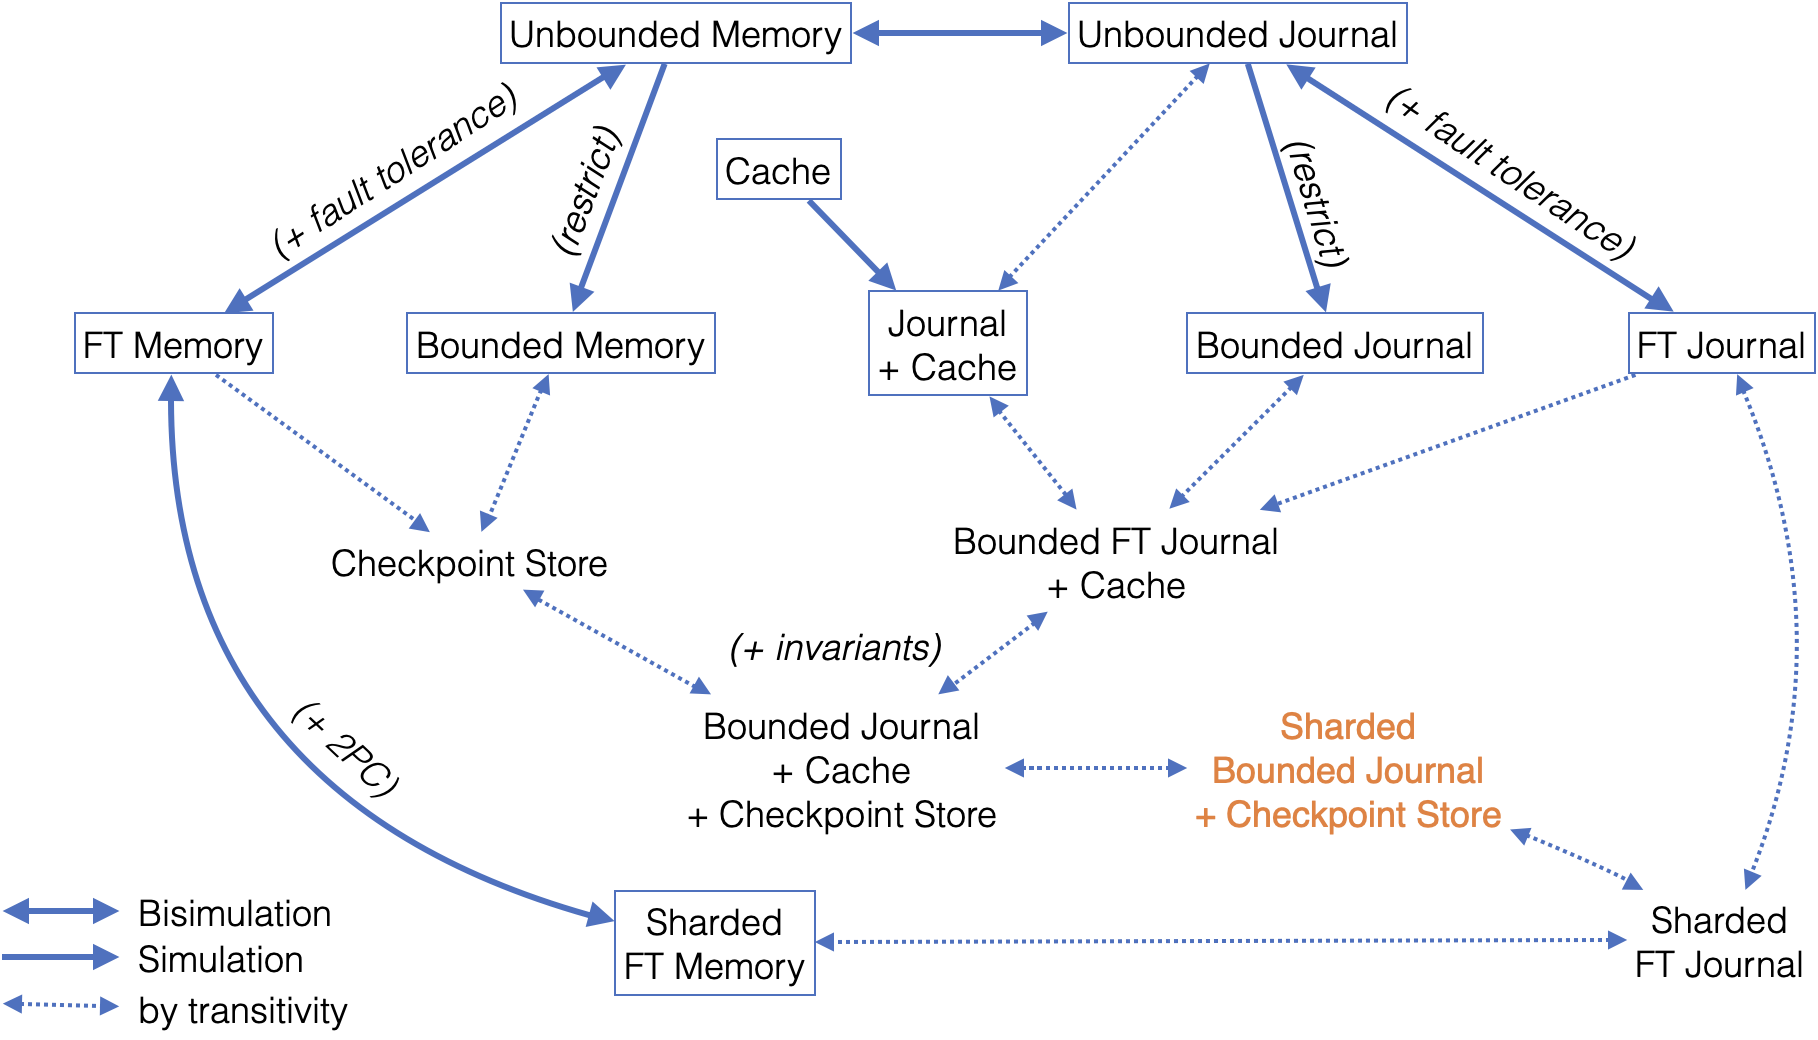
\includegraphics[width=0.75\textwidth]{figures/transitions.png}
  \caption{Needs to be changed}
  \label{fig:transitions}
\end{figure}

\subsection{Transactional Causal Consistency (TCC)}

Our model supports multiple consistency levels. In this work however, we focus on Transactional Causal Consistency (TCC).
TCC means that: (1) if one update happens before another, they will be observed in the same order (causal consistency), and (2) updates in the same transaction are observed all-or-nothing.

To keep track of happened-before, we use timestamp to order updates.
When a transaction $\tau_i$ commits, it is assigned a commit timestamp $Ct_i$ timestamp and the effects $\varepsilon_i$ moved into the store with as object versions $(key,Ct_i)$.
These occur atomicallu with regard to any other transactions.
If a transaction $\tau_j$ has a dependency $Dt_j$ higher than $Ct_i$ than all the effects of $\tau_i$ are visible for $\tau_j$.

Reformuler en expliquant pourquoi les CRDT ici(Conflits are taken care of by using CRDTs as our data type ensuring that reading from a snapshot $St$ is determistic.)

We introduce our first system invariant:

\[
  \begin{array}{lcl}
    \emph{$Dt_i < Ct_i$}
  \end{array} 
\]

\section{Intuitive model}

We start with an intuitive simple in-memory key-value store.
Therefore if a crash or restart occurs the database is lost.
In this section we present the semantics from the viewpoint of the system.
The general behavior describe in this section is as follows.
A client starts a transaction and execute a sequence of operations and tries to commit or abort the transaction.
This means all operations executed by the client must be part of a \emph{live} transaction.
This also include the commit and abort call.
Another guarantee our model provide is that for any committed transaction, the commit timestamp must be greater than the dependency timestamp.

These are the transaction invariants maintained during transactions:
\[
  \begin{array}{lcl}
    \emph{$Ct \neq null => Dt_i > Ct_i$}\\
    \emph{$(read, effect, commit, abort) => State = live$}
  \end{array} 
\]



\textbf{Start transaction} (Session part missing)
When a client starts a transaction, if the client specify a dependency timestamp $Dt$ the system checks if it is valid in regards to consistency guarantees and creates a transaction object.
If no dependency timestamp is specified than system assign a valid snapshot to the transaction.
(On parle de l'implémentation de ce mécanisme plus tard)
The transaction is then assigned a unique transaction identifier $\tau_i$ and $\emph{State} \leftarrow \emph{live}$.
Here are the preconditions, invariants and postconditions:
(Alt) From these requirement we extract the following preconditions:

Preconditions:\\
$State \neq live$
$Ct = null$

Invariants:\\
\emph{$Ct \neq null => Dt_i > Ct_i$}\\
$Ct = null$

Postconditions:\\
$State_i = \emph{live}$ \\
$Ct = null$


\textbf{Read} returns the correct Object-version in the store that is valid in regads to our consistency model.
If two conccurent Object-versions exist, meaning they are part of two transaction that have a commit timestamp lower or equal than the dependency timestamp and are not related by precedence.
(NOTE: première fois que j'en parle)
We use a deterministic algorithm, ie. merge or LWW, to choose the Object-version returned.
In case there are no existing Object-version in memory we return a default value.
Finally the system adds the key to the read set $R_i$ of the transaction. 

Preconditions:\\ 
$State_i = \emph{live}$ \\
$Ct = null$

Invariants:\\
$State_i = \emph{live}$ \\
$Ct = null$

Postconditions:\\
$R_i = R \cup \{key\}$ \\

\textbf{Effect} the system creates a new Object-version by merging the Object-version that is returned by \emph{read(key)} with the effect.

Preconditions:\\ 
$State_i = \emph{live}$ \\
$Ct = null$

Invariants:\\
$State_i = \emph{live}$ \\
$Ct = null$

Postconditions:\\
$\varepsilon_i = \varepsilon_i \cup \{(key, \tau_i)\}$ \\

\textbf{Commit} the system checks if the effects $\varepsilon_i$ are valid in regards to the consistency model and abort if not. (Need more precision. Maybe earlier here does not seem to be the correct section)
If the effects are valid the Objects versions are added to the Store and assigns a commit timestamp $Ct_i$.
Finally the transaction's $State$ is set to $terminated$ making the effects visible in the store atomically.

Preconditions:\\ 
$State_i = \emph{live}$ \\
$Ct = null$

Postconditions:\\
$Store = Store \cup \varepsilon_i$\\
$State = terminated$\\
$Dt_i \geq Ct_i$.\\

\textbf{Abort} updates the state of the transaction to $terminated$ without updating the Store with the effects of the transaction and no commit timestamp is assigned

Preconditions:\\ 
$State_i = \emph{live}$ \\
$Ct = null$

Postconditions:\\
$State = terminated$\\
$Ct = null$

\subsection{Bounded Memory}

Unbounded memory is not realistic in a real system.
In the Bounded Memory model we choose to define an arbitrary limitation on the size of the memory used by the system.

\textbf{System invariants}
All system invariants from the Unbounded memory are present here.
Plus we introduce a two new value:
\begin{itemize}
  \item \emph{$M_{used}$} contains the current size of data in memory
  \item \emph{$M_{limit}$} represents the maximum size available to the database
\end{itemize}
Based on these two variable we introduce a new system invariant:
\begin{itemize}
  \item \emph{$M_{used}$} $<$ \emph{$M_{limit}$}
\end{itemize}
In order to uphold the memory constraints of the system we keep track of all the dependencies of running transactions called \emph{RunningTr} but also all the commit timestamps of finished transactions \emph{CommitTr}.

We then introduce a new timestamp called Minimum Dependency \emph{MinDt}.
\emph{MinDt} represents the oldest snapshot any running transaction is reading from.
When a transaction $\tau_i$ commits or aborts, it is removed from \emph{RunningTr}. 
And if $Dt_i = MinDt$ and no other transaction is reading from $Dt_i$ the system advances \emph{MinDt} to the next oldest snapshot used in \emph{RunningTr}.

\subsection{Garbage collectio - WIP}
When \emph{$M_{used}$} $\geq$ \emph{$M_{limit}$}. 
All the transaction in the system are halted in order to perform a garbage collection.

Ici je dois expliquer comment est fait le GC:\\
\begin{algorithm}
  \KwIn{\\ \Indp
    RunningTr : set
  }
  \(oldTr \longleftarrow \emptyset\)\;
  \ForAll{\(\tau_{i} \in Running\)}{
    \If{\(Dt_{i} < MinDt\)}{
      \(oldTr \longleftarrow \tau_i\)\;
    }
  }
\end{algorithm}

WIP


\subsection{Implementation - WIP}

Every model is implemented in java with external libraries for persistency, CRDTs and data structures that we consider being correct.
Implementation and evaluation of the different models have two purposes.
First we implement our different models as closely as possible to our specification and show that they are correct by running the same test on all versions.

Finally we plan on designing test that specifically targets breaking invariants defined in our model making sure the system crashes if they are violated, and run a set of traces that are generated from a Coq implementation.



\section{Conclusion}


\bibliography{exemple,predef,shapiro-bib-ext,shapiro-bib-perso}

\end{document}